% =============================================================================
% Section 4.4: Course Management Module
% =============================================================================

\section{Course Management Module}
\label{sec:course-module}

\subsection{Functional Description}

The Courses module manages the curriculum lifecycle: instructors create courses, organise them into modules and lessons, attach video assets and quizzes to lessons, and publish the result for learner enrollment. The module is the content backbone of the platform, and its aggregate design must support deep nesting (course $\rightarrow$ module $\rightarrow$ lesson), reordering, versioning, and concurrent editing.

The module exposes REST endpoints for CRUD operations on courses, modules, and lessons, with dedicated endpoints for publishing/unpublishing, reordering, and category assignment.

\subsection{DDD Aggregate Design: Course--Module--Lesson Hierarchy}

The aggregate root is \texttt{CourseEntity}, which owns a collection of \texttt{CourseModuleEntity} value objects, each of which owns a collection of \texttt{LessonEntity} entities. The hierarchy is enforced by the aggregate root: all operations that modify modules or lessons must go through \texttt{CourseEntity} methods.

\begin{lstlisting}[caption=Course Aggregate Root,label=lst:course-aggregate]
export class CourseEntity {
  private constructor(
    public readonly id: string,
    public title: string,
    public description: string,
    public instructorId: string,
    public price: Money,
    public status: CourseStatus,
    public modules: CourseModuleEntity[],
    public version: number,
    public categoryId: string,
    public thumbnailUrl?: string,
  ) {}

  static create(props: CreateCourseProps): CourseEntity {
    return new CourseEntity(
      props.id, props.title, props.description,
      props.instructorId, props.price, CourseStatus.DRAFT,
      [], 1, props.categoryId,
    );
  }

  publish(): void {
    if (this.modules.length === 0)
      throw new BusinessRuleViolation('Course must have at least one module');
    if (this.modules.some(m => m.lessons.length === 0))
      throw new BusinessRuleViolation('Each module must have at least one lesson');
    if (!this.thumbnailUrl)
      throw new BusinessRuleViolation('Course must have a thumbnail');
    this.status = CourseStatus.PUBLISHED;
    this.version++;
  }

  reorderModules(moduleIds: string[]): void {
    const ordered = moduleIds.map(id => {
      const mod = this.modules.find(m => m.id === id);
      if (!mod) throw new BusinessRuleViolation(`Module ${id} not found`);
      return mod;
    });
    this.modules = ordered.map((m, i) => m.withPosition(i + 1));
    this.version++;
  }
}
\end{lstlisting}

The aggregate enforces three invariants at publication time: a course must have at least one module, every module must have at least one lesson, and a thumbnail must be set. These rules are checked in the \texttt{publish()} method and cannot be bypassed by external code.

\subsection{Optimistic Concurrency Control}

Each \texttt{CourseEntity} carries a \texttt{version} field that is incremented on every mutating operation. The Prisma repository implementation includes the version in the WHERE clause of the write query:

\begin{lstlisting}[caption=Optimistic Concurrency Update,label=lst:optimistic-lock]
async update(course: CourseEntity): Promise<void> {
  const result = await this.prisma.course.updateMany({
    where: { id: course.id, version: course.version - 1 },
    data: {
      title: course.title,
      status: course.status,
      modules: { deleteMany: {}, create: this.serializeModules(course) },
      version: course.version,
    },
  });

  if (result.count === 0)
    throw new ConcurrentModificationError(
      `Course ${course.id} was modified by another transaction`
    );
}
\end{lstlisting}

If two instructors open the same course, both modify it, and both submit their changes, the second write will match zero rows (because the version has been incremented by the first write) and the repository throws \texttt{ConcurrentModificationError}. The use case can catch this error and present the instructor with a conflict-resolution dialogue. This pattern avoids pessimistic locking (SELECT FOR UPDATE) which would block read access to course content during editing --- an unacceptable trade-off given that concurrent read access by enrolled learners is the common case.

\subsection{Idempotency for Lesson and Module Operations}

All mutating endpoints in the Courses module accept an optional \texttt{Idempotency-Key} header. The system maintains an idempotency ledger table (\texttt{course\_idempotency\_keys}) keyed by the SHA-256 hash of the key. If the same key is received within a configurable time window (default 24 hours), the response from the first request is returned without re-executing the operation. This is essential for mobile clients on unreliable networks, where a create-lesson request might succeed but the client never receives the response and retries, potentially creating duplicate lessons.

The course curriculum lifecycle is summarised by the state machine in Figure~\ref{fig:course-statemachine} showing transitions between DRAFT, UNDER\_REVIEW, PUBLISHED, and ARCHIVED.

\begin{figure}[H]
  \centering
  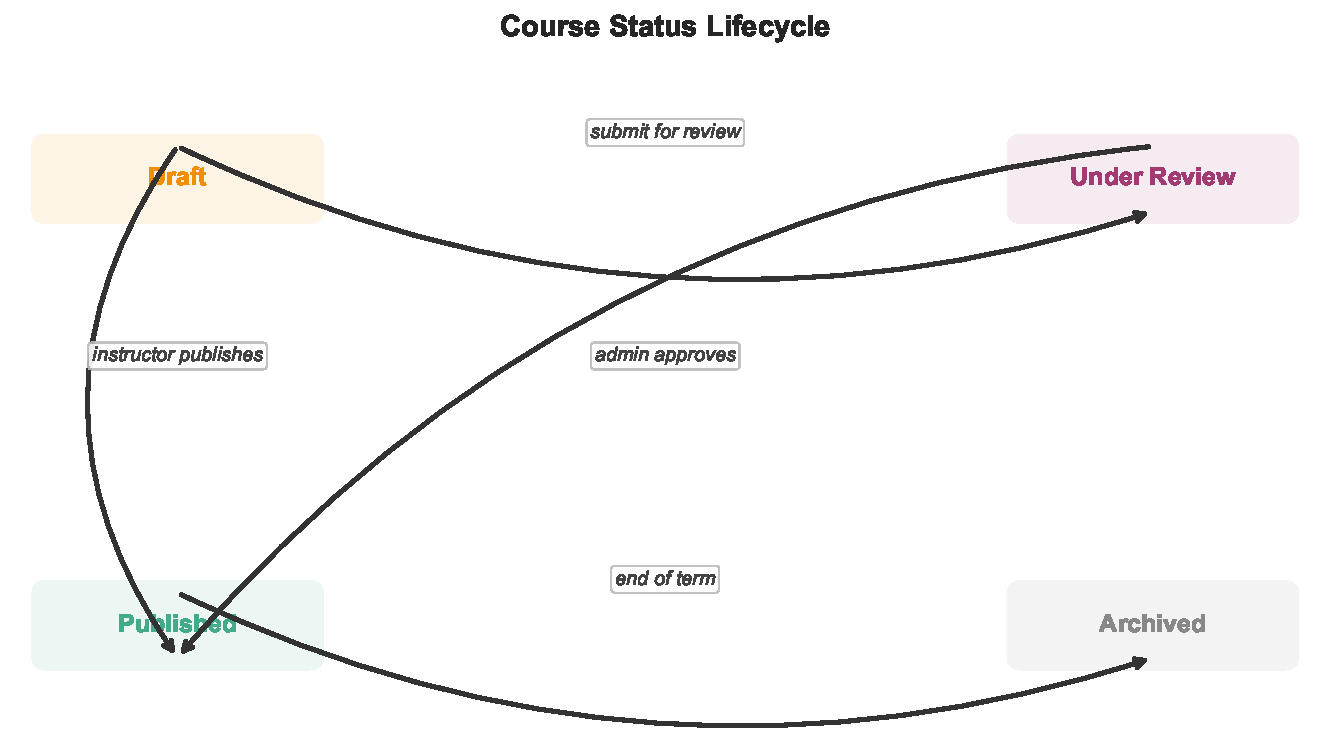
\includegraphics[width=0.55\textwidth]{images/statemachines/course_curriculum_statemachine.pdf}
  \caption{Course Status Lifecycle}
  \label{fig:course-statemachine}
\end{figure}
